\section*{Motivation}

%%<why do opvs matter>
The global climate crisis is one of the most pressing issue humanity faces today.
Consumption of fossil fuels for energy and transportation strongly contributes to atmospheric $CO_2$ the affects of which are global, long-term, and devastating\cite{Solomon2009a}.
In our technology-driven society, it is unrealistic to think that energy demand will lessen, in fact global energy consumption is predicted to increase from 17 TW in 2010 to 27 TW in 2040\cite{Mazzio2015}.
In order to protect our climate, we need a non-polluting, cost-efficient way to provide electricity.
Harnessing solar energy is an important part of a green energy solution.
Renewable energy accounts for 11\% of the U.S. energy consumption in 2019 and of that 11\% 9\% was solar\cite{USEIA2020}.
Our energy infrastructure has room for improvement: consider Germany which in 2019 got 43\% of its energy from renewables and 8.2\% of its total energy from solar\cite{Wirth2017}.
Traditionally, photovoltaic devices, materials which can convert incedent light into electric current, were made of inorganic materials like silicon.
But in the late 1970's organic photovaltaics (OPVs) were discovered as a potential alternative\cite{Tang1986b}.
The advantage of OPVs over inorganic PV devices is that OPVs are lightweight, low cost, easier to produce, and flexible. 
However, in order to become a viable, cost-effective option they need better efficiency\cite{Mazzio2015}.

\begin{figure}[h!]
    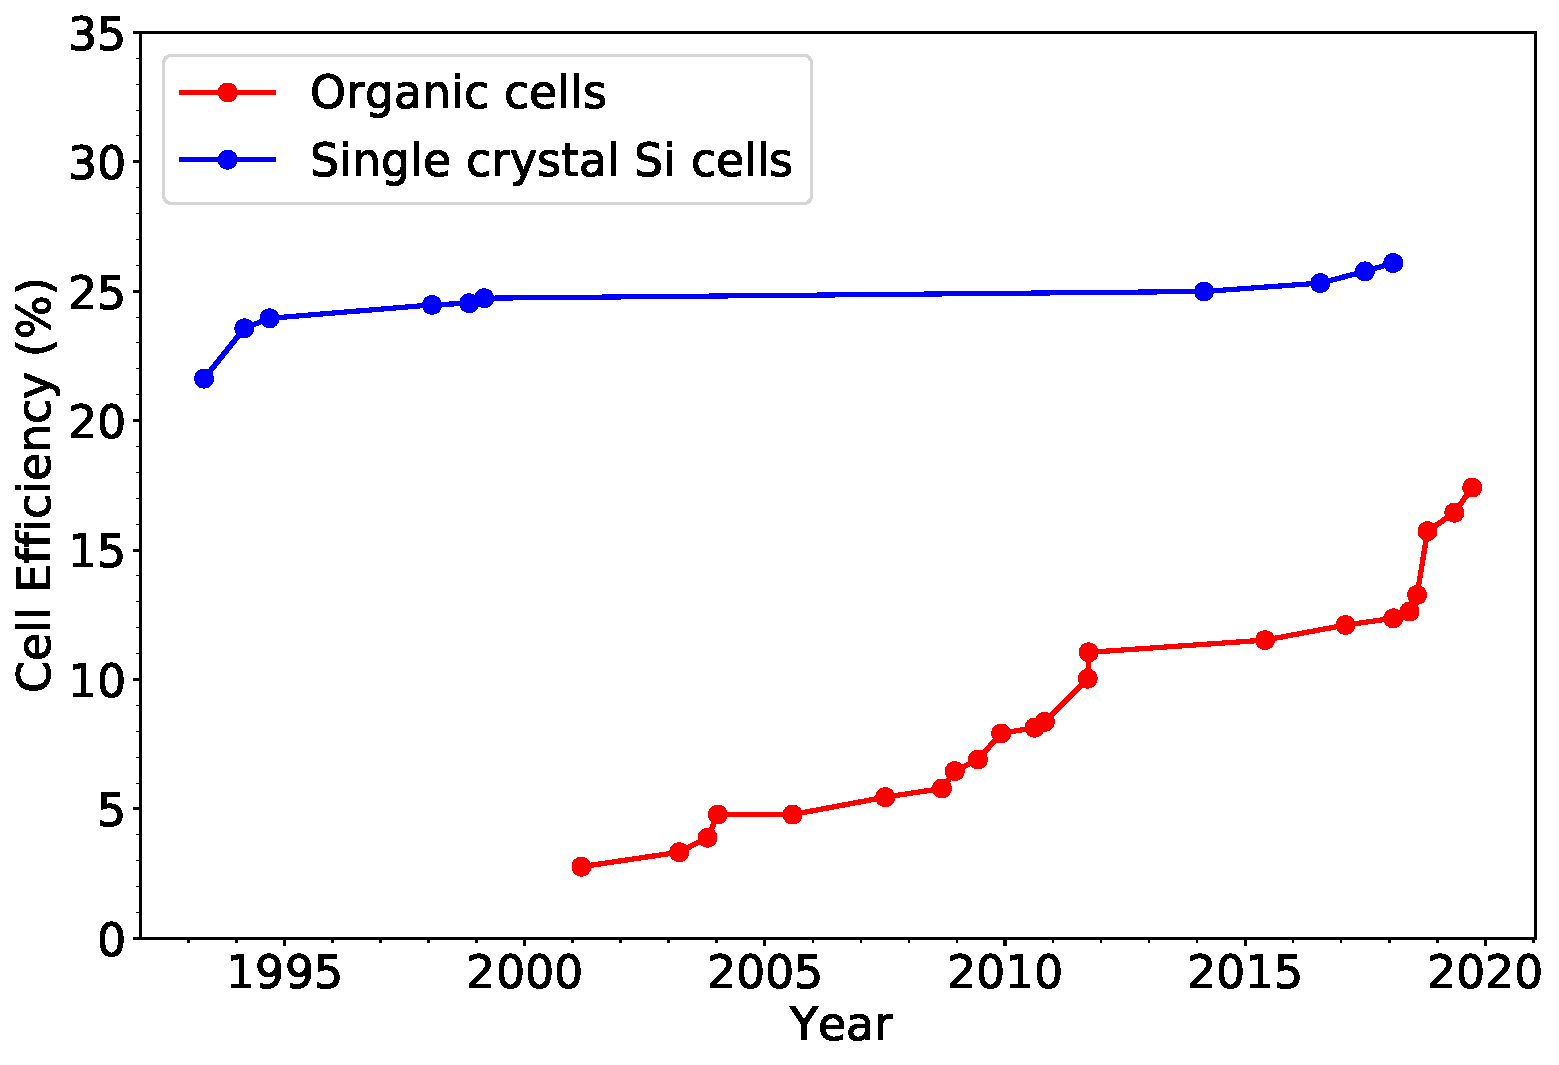
\includegraphics[width=0.9\linewidth]{images/NREL2020.pdf}
    \caption{Efficiencies of photovoltaic technologies from 1976 to present. OPVS are denoted by red filled circles. The current state-of-the-art research cell achieves 17.4\% efficiency. Image taken from ref \cite{NREL2020}}
    \label{fig:nrel}
\end{figure}

In order to make the most efficient OPVs we need to find the best blend of compounds and the processing conditions that result in the best structure for those compounds.

The active layer of an OPV is mixture of electron-donor and acceptor compounds: the ideal morphology is a micro phase-separated interpenetrating network called a bulk heterojunction (BHJ).
The performance of an OPV device is intimately linked with the structure of the active layer:
With minor modifcations, the number of compounds and the processing conditions can become infinite which makes this an intractable problem for experiment.
Imagine, you are a chemist synthesizing and testing new OPV morphologies: you are specifically looking at a mixture of a non-fullerene acceptor, \textit{3,9-bis(2-ethylene-(3-(1,1-dicyanomethylene)-indanone))-5,5,11,11-tetrakis(4-hexylphenyl)-dithieno(2,3-d:2',3'-d')-s-indaceno(1,2-b:5,6-b')dithiophene} (\textbf{ITIC}), and a polymer donor, \textit{poly((4,8-bis((2ethylhexyl)oxy)benzo(1,2-b:4,5-b')dithiophene-2,6-diyl)(3-fluoro-2-((2-ethylhexyl)carbonyl)thieno(3,4-b)thiophenediyl))} (\textbf{PTB7}). 
Each compound costs \$500 for 100 mg\cite{sigmaaldrich}.
The solvent you use and the concentrations of your active compounds changes the device performance\cite{Hoppe2004a}.
The amount of time the solvent is allowed to evaporate changes the device performance\cite{Li2007}.
The time and temperature of the thermal annealing changes the device performance\cite{Ma2005}.
The regioregularity of your polymer affects the device performance\cite{Kim2006}.
The distribution of polymer lengths affects the device performance\cite{Zhao2013b}.
Changing the functional groups on ITIC changes how it packs in a crystal, its electron affinity, and thus its performance in a device\cite{Swick2019a}.
All this would be to determine the performance of just one donor/acceptor combination in one category of potential compounds\cite{Dou2013}.
By using a simulation pipeline, we can help to streamline the process of determining which OPV materials will form the best morphology with the best charge transport, and in turn, help to solve the energy crisis.

Molecular simulation also gives us insight into the atomic interactions which drive the self assembly of an OPV morphology.
A complication of the simulation of OPV polymers is that the properties which predict a device's efficiency, for example charge transport, span multiple length scales.
The atomic and electronic properties are important for light absorption, in which an exciton is created, and charge transfer, where the exciton is dissociated into a free electron and hole\cite{Scharber2006a,Hoppe2004,Mazzio2015}.
At the same time, the exciton finding an interface at which to dissociates depends on the bulk morphology, as do the charges, once separated, finding a path to an electrode in order to generate current and produce electricity.
So, in order to model this system, a multiscale approach is necessary.
By breaking our simulation apart into separate steps and equilibrating different lengths scales individually, we can get equilibrated morphologies on multiple length scales more efficiently.

Already good open-source packages exist to address the problem of coarse-graining and/or backmapping\cite{Marrink2007,Ruhle2009,Maerzke2011,MorphCT,Wassenaar2014b}. %%these citations are martini, votca, trappe, morphct, backwards.py
By making code open source and freely availiable, we contribute to the knowledge of a global community. 
But just because something is availiable doesn't mean it is accessible: often just figuring out how to use an existing package can be very difficult\cite{Cummings2019}.
These existing codebases can appear to a new user as monolithic and indecipherable because their design has been to solve a problem, which they do, instead of design with a focus on how people learn.
These codebases also rely on users piecing together multiple, often incompatible, bits of software, using manually created xml files, or manually deciding how to classify a atom grouping based on the users chemical intuition.
All of which contribute to a reproducibility crisis in the computational sciences\cite{Baker2016}.
By keeping best practices for software development and teaching in mind throughout development, we can strive to make tools which make science more transferrable, reproducibile, usable, and extensible (TRUE)\cite{Thompson2020}. %%TRUE
Best software development practices include using version control software, such as git, to facilitate the process of tracking and merging changes to a code repository, especially important when working collaboratively.
Also among these best practices are using unit tests and continuous integration to ensure that errors are quickly and automatically caught\cite{Wilson2014}.
Instead of writing dense, inseparable scripts which rely on the user manually following a command prompt or editing multiple text files, we aim to keep code small and modular to make it easier to use and understand\cite{Adorf2018a}.
Following these guidelines not only makes our code easier to develop and debug, but reduces the cognitive load for a new user\cite{Jankowski2019}.
Providing good documentation and tutorials is also imperative for onboarding new users.
Jupyter Notebooks, which are a combination of interactive code and formatted text and images, can be used like a lab notebook for computational scientists in order to demonstrate the process, rationale, and the story of each experiment and the exact steps to get the results shown\cite{Rule2019a}.
When writing these tutorials, it is wise to remember that the data never speaks for itself: although including input and output files of a calculation is a good first step, they must be accompanied by the story of what the data means and how a user can know that meaning for themselves\cite{SWC, Wilson2016}.

Use flexible method for specifying coarse grain models to obtain OPV polymer morphologies equilibrated on length scales relevant to charge transport.
Use a backmapping method, which works on the same simple mapping operator, to restore the atomic positions in preparation for techniques which require atomic level resolutiuon e.g., charge transport calculations.
This two step process is necessary because starting with the fully atomistic structure would not only be computationally inefficient the result may even be less accurate due to the difficulties of equilibrating polymers\cite{Gartner2019a}.
This efficiency is important because the scope of potential OPV compounds is vast and the energy crisis necessitates expediency.
The number of opv compounds to test quickly becomes intractable when we consider that the power conversion efficiency is strongly linked to minor chemical modifications or functionalization, device processing, and the interplay between donor and acceptor\cite{Mazzio2015,Swick2019a}.
There are countless variations of electron donor polymers, fullerene acceptors, and more recently small molecule, non-fullerene acceptors (NFAs) have been recieving attention for their potential to achieve higher efficiencies\cite{Dou2013}.
A P3HT:NFA blend was shown to have 11\% PCE, compared to the state-of-the-art 6.4\% in P3HT:PCBM\cite{Baran2017}.
Not only are NFAs found to be more efficient, but they also show to be more stabile in air than polymer:fullerene blends (retaining 70-80\% of the PCE after 1,200 h exposed to air while the fullerene device was no longer operational after 800 h)\cite{Baran2017}.
Coarse grain models do not yet exist for many of these NFAs, and with so many varieties an adaptable pipeline makes more sense than a single model.%%<there aren't a lot of cg models that already exist for these new compounds>
It is necessary to develop a simple, useable, and flexible pipeline to adapt to the constantly changing chemistries of current OPV technologies. %EJ: NIIICE SENTENCE.

\section*{Research Objectives}

%EJ: Nice. Attempting to reorder based on heirarchy
%%use that science to help solve energy crisis???????>
Ultimately the goal this research is to help solve the global energy crisis. 
Solar energy is a important part of a green energy solution.
This research aims to gain insight about new OPV compound morphologies using molecular simulation.

%%create models for new opv compounds>
In order to model these OPV polymer systems on relevant length scales, it is necessary to develop new coarse grain models.
A flexible and efficient coarse graining scheme will simplify the process of mapping and parameterizing (these coarse grain elements). %% reword

%%gain insight into the limits of coarse graining>
The flexibility of specifying a mapping will allow for the comparison of multiple mappings which may provide insight into the features of an OPV which govern its self-assembly and the limits of coarse grain models.
Currently there is no agreed-upon ``best'' scheme for a coarse grain mapping operator.
By making a simple and easy-to-use coarse graining tool, many mapping operators can be tested and the limits of a minimal model can be probed.
%% What is the minimum structure needed to represent a complex molecule? %% reword? omit?

%%develop new tools that help humans do science>
Making this tool usable will also hopefully contribute to reproducibile science. 
Integrating with existing open source software packages will provide the most benefit and also increase transferrability and usability.
We will use packages like signac for managing dataspaces, foyer for version control of forcefields, mbuild for building chemical structures, hoomd for running molecular dynamics simulations, freud for simulation trajectory analysis, and openbabel for recognizing chemical patterns. %%cite!
These are established codebases which are actively developed and engine agnostic (except hoomd which is in itself an engine).

%%create a workflow that will make creating new models more accessible>
Demonstrating a workflow from start to finish with explanations using easy-to-understand language, diagrams, and figures makes a codebase more usable and approachable but does not interfere with it being modular or efficient.
Ultimately a goal of this research is that it is used by others: as an example to build upon or as a template for setting up their own experiments.

\section*{Background}

\subsection*{Organic Photovoltaics}

%% <what is PCE>
The power conversion efficiency (PCE or sometimes $\eta_{e}$) is the ratio of electrical power produced by the device over the power of incedent photons.
Higher PCE means the device is more efficient.  
The material properties which determine the PCE of a device are those which affect the number of photons absorbed, excitons dissociated, and free charges that reach the electrode.
The absorption efficiency depends on the absorption spectrum, absorption coefficient, and layer thickness.
The fraction of excitons which dissociate depends on the exciton dissociation length and the charge separation probability at the interface.
Finally, the the number of charges which reach the electrode depends on the driving force or gradient resulting from the potentials of the electrons and holes\cite{Hoppe2004}.
%%<is there a citation for why charge transport is a good proxy for PCE?>

%% <history>
Inorganic PV devices came first and are still most efficient, but they are more costly to produce, use rare elements, and their production causes other environmental issues, so they aren't the best solution for solar energy harvesting. 
The first OPV was created by Tang in 1986 and used a bilyaer structure containing copper phthalocyanine and a perylene derivitive\cite{Tang1986b}. 
This early device had a PCE of 0.95\%.
In 1992, Saricifti and Heeger were the first to report using fullerene as an electron acceptor in a fullerene:polymer mixture\cite{Sariciftci1992}.
And in 1995, Yu described the first bulk heterojunction (BHJ), as an interpenetrating network of donor and acceptor that maximizes the interfacial area, which is still the state of the art morphology to this day\cite{Yu1995}.
Most recently, non-fullerene acceptors (NFAs), like ITIC, are contributing to the PCE increase of modern OPVs\cite{S.Gurney2019b}.

\begin{wrapfigure}{L}{0.5\linewidth}
    \centering
    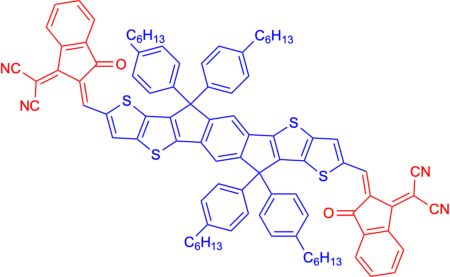
\includegraphics[width=0.6\linewidth]{images/ITIC.pdf}
    \caption{ITIC chemical structure with \textcolor{red}{electron accepting regions in red} and \textcolor{blue}{electron donating regions in blue}}
    \label{fig:itic}
\end{wrapfigure}

The planar acceptor-donor-acceptor moeity seen in many NFA backbones (see Figure \ref{fig:itic}) may have more efficient exciton splitting, as compared to a fullerene acceptor, at the heterojunction due to strong electronic coupling between the conjugated backbones of the NFA and the polymer\cite{Yi2018a}.

%%<how opvs work>
The compounds which compose an OPV are synthesizable molecules (often polymers) composed of abundant elements (carbon, hydrogen, nitrogen, sulfur, oxygen).
Due to the conjugated pi-orbitals in these molecules the absorption of sunlight can excite an electron into a frontier orbital and generate an exciton.
OPVs are made as a mixture of electron-donor and electron-acceptor compounds in a structure called a bulk-heterojunction.
Depending on the bulk morphology of these compounds, the exciton can travel to an acceptor-donor interface and dissociate into free electron and hole then these free charges generate current if they can subsequently make their way to an electrode.

%%<why morphology matters>
The morphology of the device can be affected by the processing conditions: temperature, solvents, and concentrations/ratios of the active compounds\cite{Ma2005,Hoppe2004a,Li2007}.
The interfacial area of the acceptor:donor regions\cite{Mazzio2015}, the regioregularity of the polymer\cite{Kim2006}, and electronic properties of the compounds\cite{Scharber2006a} all play an important role in the power conversion efficiency (PCE) of the device. 
These changes in structure can strongly affect the device performance.
Molecular simulation allows us to "see" these atomic interaction and gain a deeper view into the driving forces behind the self assembly of these OPV morphologies and to understand what conditions create the best devices.
%%<segue into simulation>

\subsection*{Molecular Dynamics}
%EJ: Here or above: Why MD the right tool?
%% morphology matters - thermodynamics that govern self assembly
%% the kinetics that follow the processing
%% we can see the dynamics -- kinetic arresting, (if we want to probe the processing, need the dynamics)
%% monte carlo inefficient for polymers - cluster moves, not parallelizable 
%%<I am borrowing heavily from Mike's MD section, so I need to come back through and rewrite this>
%%<md in general>
classical physics
interactions between particles
non bonded/bonded/angles/dihedrals
integrates Newton's equations of motion to update the particle positions.
iterated until thermodynamic equilibrium
sample a thermodynamic ensemble
First MD simulation system of 108 particles, 200 collisions in one hour on an IBM-704\cite{Alder1957}.
Now GPUs 100 millions times faster
%%<what is MD used for? why is MD the best technique for gettign these OPV morphologies?>
protein folding \cite{levitt75}, other biological processes, polymers \cite{Gartner2019a}


%%<what assumptions does md make?>
bonds aren't formed or broken, electrons don't exist
hydrogen bonding
dispersion is tricky--electrons don't slosh around unless you use some fancy many-body potential
%%<what are the limits of atomistic md?>
%%<segue to why we need CG models>

\subsection*{Coarse Grain Models}

Coarse-graining refers to grouping atoms in a structure into a "super-atom" and using an effective potential to represent the resulting coarse grain site.
Coarse-grain models allow for simulators to access length and time scales that would be otherwise impossible using atomistic models.
%%<how do cg models let us access long length/time??>
Similarly to how we don't need to look at the working of a plant cell to understand the growth of a forest, we don't need to consider atomic level properties when we are interested in the bulk morphology\cite{Muller-Plathe2002}.
The heart of coarse graining is the removal of degrees of freedom. 
This effective potential used to represent the reduced system results in a smoothed free energy landscape. 
Processes which may have taken many time steps in an all atom simulation can take fewer time steps in a coarse simulation\cite{Berendsen2010}.
Due to their long length and time scales, coarse grain models are ideal for examining polymer properties\cite{Gartner2019a}.
It is too big and too slow and also just a bad idea to simulate huge boxes of atomistic polymers.
Even if the simulation was to complete, there would be too much information to process accurately. 
CGing allows scientists to FOCUS their experiments\cite{Baschnagel2000}.
The resolution of coarse grain systems is broad:
Simply grouping hydrogens with the heavy atom they are bonded to, called the united-atom model, has been shown to speed up dynamics and make polymer length scales more easily accesible\cite{Paul1995a, Yang2006a}.
Other coarse-graining schemes may group functional groups together\cite{Berendsen2010, Jankowski2013, Marsh2014}, one bead per repeat unit in a polymer\cite{Lee2011}, or even represent an entire amino acid with a single site\cite{Peng2019}.
%%<examples of cg models and the cool things they do>
General coarse grain models of opv thiophene polymers where only the spacing, regioregularity of the side chains were varied were able to predict different order disorder transitions and calculated scattering patterns of these simple systems were comparable to those obtained from experiment\cite{Jankowski2013, Marsh2014}.
A coarse-grain model for phospholipids has allowed for bilayer formation from an initial random configuration to be observed even though the model was parameterized to the vapor-liquid phase transition\cite{Shelley2001}.
Which model is right depends on the length and time scale on which the property of interest can be observed.
%%<multiscale sims>
For many systems, however, we are interested in properties which span length scales.
For instance, in a system like a opv polymer melt, it is not only computationally intractable to try and simulate the electron density on length scales proportional to the exciton dissociation length (~5-10 nm)\cite{Huang2010} -- it is the wrong tool for the job.
If what we are interested in is the properties of the polymer in the bulk heterojunction, then it is wise to abstract away any degrees of freedom which do not directly contribute to the self-assembly of the structure.
Once a good bulk structure has been achieved, the atomistic details can be reintegrated much more easily--a process called backmapping.
In the same way that a coarse grain model can be mapped onto an atomistic one, we can get a reasonable starting structure for an atomistic simulation from a coarse grain structure.
The large length scale, polymer level properties can be equilibrated during the coarse grain simulation, and then the atomic interactions can be equilibrated during the backmapped atomistic simulation.
This can allow us the calculate properties such as charge transport, which depends upon the electronic structure of individual chromophores and the connectivity of these chromophores over distances proportional to the exciton dissociation length.
%%<what stands in our way?>

%%<coarse-grain models are specific>

%%<segue from automated creation of forcefields to...>
%%<mapping operator has to be decided by hand> <is this section too big?>
Part of coarse graining that is not yet automated is choosing a mapping scheme or a mapping operator.
A mapping operator defines which atoms are grouped into a "super atom" represented by one coarse grain site and where in the site is placed relative to the atom group.
Mapping operators are chosen based on desired resolution of the coarse grain system and the information to be extracted.
A straightforward way to define a mapping operator is to group a set number of heavy atoms (non hydrogen) together--this is the method used in the MARTINI force field\cite{Marrink2007}.
In this scheme, four atoms (except rings, which are treated differently) are grouped and the site is classified as polar, non-polar, apolar, or charged depending on the atoms it is composed of.
When parameterizing a new molecule you must pick a mapping and then compare the resulting beads to existing beads--a process which is time consuming and error prone\cite{martini-tutorial}.
The MARTINI force field was first designed for lipids--further parameterization for proteins and nuclei acids have been added--and has shown to be effective in predicting vesicle formation, membrane protein dynamics, etc.%%<cite
Many mapping schemes are simply based on the user's chemical intuition (e.g., what parts of the molecule shouldn't be allowed to bend? What groups have the most dominant interactions in this structure %%<cite any model where rings are one bead><cite dna cg model>).
As the number of atoms in the fine grain structure increases, the number of possible mappings increase drastically.
There have been efforts to create mapping schemes for automating the process of deciding which atoms are grouped in a "super-atom" bead.
One study reduced the number of allowed mappings by only allowing those which do not change the symmetry group, then iterated over a graph of all possible mappings to find the "best" mapping by comparing the difference between the mapped RDF and velocity autocorrelation function\cite{Chakraborty2018b}.
Another mapping scheme uses principle component analysis to choose a mapping scheme for biomolecules that best represents th essential dynamics\cite{Zhang2008}.
Mapping operators can be automated using machine learning: clustering methods combined with graph analysis were shown to predict the "expert" mapping chosen using chemical intuition reliably\cite{Li2020}. 
A mapping operator based on the centers of charge was shown to accurately model electrostatic properties\cite{Cao2015a}.

%%<how cg potentials have been attained>

\subsection*{Multi-State Iterative Boltzmann Inversion}

There are numerous methods for deriving coarse grain potentials from atomistic ones (e.g., force-matching, reverse Monte Carlo), but in this proposal we will focus on Iterative Boltzmann Inversion (IBI).
%%<IBI>
IBI is where a coarse grain potential is iteratively tuned to fit a target distribution\cite{Reith2003}.
Here is the algorithm for determining the non-bonded potentials:
First the coarse grain system is mapped onto an equilibrated atomistic one.
Then the radial distribution function (RDF) of the mapped systems is calculated over the equilibrated frames of the trajectory--This is the target distribution.
Given any particle, the RDF gives the probability of finding a neighboring particle at distance r.
Taking the Boltzmann Inverse of the RDF results in the potential of mean force (PMF). %%<add equation>
Then a CG simulation can be run using the PMF as the non-bonded potential to achieve a new distribution.
Then the difference between the new and target distribution can be accounted for in the next iteration accoring to equation %%<add equation>.
This process is repeated until the difference between the result and the target are sufficiently similar.

The coarse grain potential derived from IBI is not transferrable to different thermodynamic statepoints.
This is because the RDF is a property of the ensemble average at a given statepoint, so the potential derived from this property is also limited.
For example, separate potentials are required to capture solid and fluid structures of a pure simple lipid \cite{Hadley2010a}.
There are many attempts to create transferrable CG potentials, for example:
The TraPPE force-field fits CG potentials using vapor-liquid equilibria to improve transferrability across thermodynamic states\cite{Maerzke2011}.
But optimization to the liquid-vapor equilibriai, although useful for prediction of thermodynamic properties, may not be ideal for prediction of structure which will strongly influence charge transport.
%%<so we probably want to create our own potentials>
%%<IBI potentials are sometimes transferrable and it is not clear why sometimes they are and sometimes they aren't.> \cite{Moore2014}

Multistate iterative Boltzmann inversion (MS IBI) includes data from multiple targets to yield a less state dependent potential\cite{Moore2014}.
The MS IBI potential is an average of the single state potentials with a weighting function to prioritize a state of interest.
This method has been shown to accurately reproduce the true potential in monoatomic LJ fluid.

When using the MS IBI method, it is important to choose dissimilar states to minimize the potential overlap region.
If this overlap region is large, there are many potentials which will provide matching RDFs. %%<show fig from moore>
For some systems there may not be a potential that represents all states-- this is not unique to coarse potentials, atomistic potentials also have this limitation.
%%<need some tie in back to why we would want to go from CG-->atomistic>

\subsection*{Mesoscale Device Simulation}

%%<I DONT WANT TO FOCUS ON THIS TOO MUCH. It's only here as a rationale for why backmapping>
%%<how morphct pipeline would work: cg-backmap-ct>
MorphCT, a software previously developed by our lab, can simulate charge transport through an OPV morphology using kinetic Monte Carlo\cite{Miller2018a,MorphCT,morphct2.2}.
The kinetic Monte Carlo algorithm used by MorphCT uses the semi-empirical Zerner's Intermediate Neglect of Differential Overlap (ZINDO/S) quantum chemical calculation to obtain the molecular energy levels of chromophores in the morphology.
The HOMO levels of each chromophore site and the energy splitting induced in the chromophore pairs is used in the Marcus equation to calculate the charge hopping rate between pairs.
A Monte Carlo simulation can then be run using these hopping rates.
Because this is a quantum chemical calculation, the position of each atom is needed--therefore a backmapping process is required to calculate the charge transport in a CG morphology.
MorphCT has some builtin backmapping tools which use xml file (which i will discuss why these are bad in the next section) and the package is bulky/CLI/hard-to-use...
%%<making morphct more modular to allow it to be used in a workflow not cli>

\section*{Preliminary Work}
% With lan - About excitonic splitting, using DFT, DNA. 
% With Matt - What intermolecular interactions guide diphenylurea crystal formation
% With us - Perspective paper about all things


%%<how do I relate this to what I want to do??>
- contributed to development of open-source packages: mbuild, foyer, signac, fresnel
 this has helped me learn best software development practices like writing documentation, using version control, writing unit tests, employing CI, fork/pull model, etc.
using these tools will help me to me a more efficient developer.
It's also helped me to learn how to work as part of a team.
 - created MWE of coarse-graining and backmapping with smiles-- these will need further testing as we try them on different compounds but the proof of concept is there.
 - created tutorial examples to help current and future students understand scientific concepts and how to use computational tools
 %% frame gixstapose as a tool for reproducible, approachable science
 - created GIXStapose (presented at SciPy2020) an interactive diffraction/structure viewer.
This may seem unrelated but we can use diffraction to verify our opv morphologies and compare them to experiment.
GIXStapose helps to beeter connect the physical structure with the diffraction pattern.
- started development on UFF repo for foyer.
This is an example of how to create a version controlled forcefield which can be automatically applied to a compound.
%%<atom typing is a pain and doing it manually is bad cite foyer paper>

%%<Talk about what exists and why it is not enough>
%%<votca, Peng2019a> 
Versatile Object-oriented Toolkit for Coarse-graining Applications (VOTCA) \cite{Ruhle2011b}
includes a coarse-graining, forcefield creation with reverse MC or IBI, and back-mapping modules.
It also allows for charge transport calculations using KMC similar to MorphCT \cite{Lukyanov2010}

reproducibility crisis.\cite{Cummings2019} \cite{Thompson2020} (TRUE paper) poorly documented code and raw data doesn't help.

instead example workflows with docker containers to build software stack.
help make science more accessible and reprodicible.

%%<compare VOTCA's backmapping to my proposed scheme>
VOTCA makes some progress towards a TRUE simulation pipeline: they include a docker container with their pre-built software stack and example input files  (but some of these input files don't work and the codecoverage on their repo as of time of writing is 0\%), and while including example inputs is a good first step, very little walkthrough (aside from code comments buried in the xml) is given\cite{votca-github}. %%using this code via docker>
A manual is provided but there is some disconnect between the example files and those given in the manual %%<https://github.com/votca/csg-manual/releases>.
the code is a mix of C++, shell commands, python, and interacts with compiled programs through the command-line and mpi.
which makes their working a little tenuous.
And judging by the amount of confusion in their mailing list %%<https://groups.google.com/forum/\#!forum/votca> there is room for improvement in the API.
Overall though this is program has many features, interfaces with many popular MD engines (lammps, gromacs, hoomd), and is under active, collaborative development.
A good question might be if I'm so into OSS and collaboration--why don't I just contribute an MSIBI package to VOTCA.
This is a reasonable question.
The answer is because I find VOTCA to be near-overwhelming in it's scope and the cognitive load of trying to fit this whole project into my brain is not ideal.
I also don't like their API.
by choosing a pure python API I will be able to make use of jupyter notebooks which can be run on cloud servers using tools like mybinder %%<link mybinder, link to tutorials I;ve made> which can combine executable code with markdown text and images.
In this way a tutorial can provide exact commands needed to reproduce the example intimately connected with the rationale and justification of that example.
I would like to think that my code speaks for itself, but after reading other people's code, I have a renewed appreciation for explanations in paragraph form, diagrams, and figures.

For an example of what I mean by cognitive load, let's compare an example of my proposed coarse-graining scheme to VOTCAs.
In the following example we will take a hexane molecule and map it to three coarse grain sites (two carbon atoms per site).


\begin{wrapfigure}{L}{0.5\linewidth}
    \centering
    \includegraphics[width=0.6\linewidth]{images/hexane-compare.pdf}
    \caption{top: hexane chemical structure, bottom: hexane overlaid with coarse grain mapping \textcolor{blue}{A}-\textcolor{orange}{B}-}\textcolor{blue}{A}
    \label{fig:hexane}
\end{wrapfigure}

VOTCA uses an xml file to do this:

%%\lstinputlisting[breaklines]{hexane.xml}

\begin{wrapfigure}{L}{0.5\linewidth}
    \centering
    \includegraphics[width=0.6\linewidth]{images/hexanexml.pdf}
    \caption{XML file used by VOTCA to specify a three site coarse grain mapping of n-hexane}
    \label{fig:hexanexml}
\end{wrapfigure}

It may be easy to think that because what we are doing--mapping two carbons and their attached hydrogens to a single bead so that six alkyl carbons becomes A-B-A--that the process will also be simple.
In order to specify a bead-mapping, we need to know the residue number, the residue name, and the atom name.
For a six atom system this is not too bad, but this could get tedious and error-prone for larger systems.
And keep in mind that these xml files need to be created manually for each compound which is backmapped.
VOTCA's scheme also requires that you specify the bonding and the angles resulting from those bonds, another process which is tedious, error-prone, and probably unecessary--I will discuss this more after discussing my scheme below:
\begin{lstlisting}
hexane_sites = [("_A", "C[CH3]"), ("_B", "CC")]
\end{lstlisting}
The result of using this code in the `coarse` function is a three-site hexane model A-B-A, same as VOTCA.%%<link to grits>
The mapping here is specified as a list of bead name / smarts string pairs.
Although they do add some element of cognitive load, SMARTS strings are designed to be human and machine readable and can match atoms based on their chemical environment.
With this scheme, there is no need to look up the name or number of each residue, I simply specify that want two alkyl carbons (using the SMARTS string "CC") and requiring that one be a terminal carbon by including that it has three attached hydrogens ("[CH3]").
The order of the beads here matters--because technically all atoms could be mapped with the more general SMARTS string (CC), it is important to list the most specific strings first.
The bonding and angles of the resulting coarse grain beads is then inferred based on the bonding of the mapped atoms.
Basically what VOTCA's xml file does in 51 lines, I can do in 1 which is easier to read and makes chemical sense. 
There are even benefits to the mapping being inline with the code:
This allows the user to see the mapping as they progress through the workflow without having to search for multiple files and it may prevent common errors caused by manual file IO such as operating system specific line endings or whitespace characters like tab or space being treated differently.
Having the mapping in-line with the workflow also allows for the user to check that the mapping is correct with built in interactive visualizations, which can display the mapping as an overlay. %%<show overlay>

We do not propose a new automated mapping, but instead a way to make the mapping and backmapping process easier for the user.
Simplified Molecular Input Line Entry System or SMILES was designed to represent organic molecules in an unambiguous way (similar to IUPAC) but in a line-entry system which is also readable by a computer\cite{Weininger1988}.
This makes it a good candidate for specifying a coarse-grain mapping scheme.The open-source package, Openbabel, allows for a SMILES string to be converted to a chemical structure and vice versa.
SMARTS is similar to SMILES but instead of representing a single molecule unambiguously, it has multiple wildcards which can be used for pattern matching.%%<cite openbabel,SMILES, SMARTS>
This pattern matching is also implemented in the Openbabel package.
If we know the SMARTS string for any given CG mapping, we can map the CG site to its center of mass or geometric center.
I have developed a minimum working example of how this can be done and then how the atomistic structure can be recovered.%%<cite grits>
It could be fairly straightforward to implement a lookup to check if bead parameters already exist--say for the MARTINI model-- by going through and writing out the SMARTS pattern for each existing bead type.
An initial headache that could make parameterizing new compounds for the MARTINI method more foolproof.

\section*{Research Plan}

- I will build on existing tools (signac,freud,mbuild,foyer,tim moore's msibi)
- create signac workflow which takes equilibrated atomistic trajectory (maybe checks if it's equilibrated?) maps the CG beads to it, runs IBI, gets tabulated FF, creates larger CG sim, runs it, does backmapping, then could do: RDF, charge transport, diffraction...
if this workflow is streamlined--it can be applied to many different compounds allowing for us to compare the analyses between our zoo of compounds.
- maybe the workflow could even involve getting the equilibrated trajectory (atomtyping/fill box/run) with the new hoomd 3 api we could even set decorrelation time as a stop trigger...

\subsection*{Objective 1: Develop a coarse graining workflow}

build on existing tools (mbuild, openbabel, tim moores MSIBI code, hoomd, foyer?)
use SMARTS matching to specify mapping operators with relative ease
use MSIBI to parameterize forcefield parameters

\subsection*{Objective 2: Develop a backmapping workflow}

Given an equilibrated CG morphology, retrieve the atomistic one by mapping the SMARTS structures onto the position of the CG beads and then relaxing them with some position restraint. 

\subsection*{Objective 3: Run CG simulation sweep of non-fullerene acceptor blends}

use signac to organize data
I think there are not great CG models for these compounds (ITIC PTB7) I found this paper \cite{Meng2019} that claims to do CGMD with PTB7 ITIC but the details are hidden in the SI and seem fishy. seems like they use IBI but they dont say how they got their target distributions.
can easily test out different mappings and "processing" conditions

\subsection*{Objective 4: Analysis}

Use charge transfer, diffraction to tell which models are the best
%%<cite a bunch of experimental papers we can compare to>
%%<cite our papers that show we can do this comparison already>
Our morphct paper says the mobilities we predict are 2x higher than experiment? why?

%%<I need something in here about making morphct more user friendly and less hard-coded for p3ht.>
%%<adding in calculation of reorganization energy??> 
%%<or just ripping out the KMC bit and making it modular>

\section*{Predicted Outcomes}

- understanding coarse graining (i'm stealing this from mike because I like it) how coarse is too coarse? for these new systems what is the minimal model which can reproduce the structural features
- understanding the interactions which guide BHJ self assembly. understanding which functionalizations/processing conditions make best morphology
- are smarts strings viable for use as mappings? where does using smarts strings break down?
- does making science easier/more understandable make it better? 


\section*{Contingency Analysis}

%%<what's going to be hard?> 
maybe SMARTS SMILES won't work without careful choice of beads. This is a little annoying but still preferrable I think because at least the reasons may be understandable (the order of the beads matters) or chemically sensible (one SMILES string may contain another -- just as one chemical moeity may be composed of more submoeities %%<this is a word?>)
coarse-graining NFAs might be hard--planar backbones and floppy side chains

\section*{Timeline for Implementation and Evaluation}
\begin{table}[h]
    \resizebox{\columnwidth}{!}{
%\resizebox{\textwidth}{!}
    %\centering
    \renewcommand{\arraystretch}{1.1}
    \begin{tabular}{| c | c | c | c | c | c | c | c | c | c | c | c | c | c | c | c | c | c | c | c | c |}
        \hline
        \multirow{2}{*}{PROJECT TASK}& \multicolumn{4}{c}{YEAR 1} &  \multicolumn{4}{|c}{YEAR 2} & \multicolumn{4}{|c}{YEAR 3} & \multicolumn{4}{|c|}{YEAR 4} & \multicolumn{4}{c|}{YEAR 5} \\ 
        \hhline{~--------------------}
             & 1  & 2  & 3  & 4  & 1  & 2  & 3  & 4  & 1  & 2  & 3  & 4  & 1  & 2  & 3  & 4 & 1  & 2  & 3  & 4\\
        \hline
           Complete Coursework & \multicolumn{10}{|c|}{ {\cellcolor{lgray}} } &  &  &  &  &  &  &  &  &  &\\
        \hline
           Present at a Conference  &  &  &  &  &  &  &  &  &  &  & x &  &  &  &  &  &  &  &  &\\
        \hline
           Publish a First Author Paper  &  &  &  &  &  & x  &  &  &  &  &  &  &  &  &  &  &  &  &  &\\
        \hline
           Proposal and Comprehensive Exam  &  &  &  &  &  &  &  &  &  &  &  & * &  &  &  &  &  &  &  &\\
        \hline
           Expand Functionality of Open Source Packages & & & & & & \multicolumn{11}{|c|}{{\cellcolor{lgray}}} & & & &\\
        \hline
           Develop Coarse Graining Package              & & & & & & & & & \multicolumn{8}{|c|}{{\cellcolor{lgray}}} & & & &\\
        \hline
           Develop Automated MS-IBI Code                & & & & & & & & & \multicolumn{8}{|c|}{{\cellcolor{lgray}}} & & & &\\
        \hline
           Develop Backmapping Package                  & & & & & & & & & & & & \multicolumn{5}{|c|}{{\cellcolor{lgray}}}& & & &\\
        \hline
           Generate Coarse-Grain Morphologies           & & & & & & & & & & & & & & \multicolumn{4}{|c|}{{\cellcolor{lgray}}}& & &\\
        \hline
           Evaluate OPV Device Performance & & & & & & & & & & & & & & \multicolumn{4}{|c|}{{\cellcolor{lgray}}} & & &\\
        \hline
           Write Dissertation & & & & & & & & & & & & & & & &{\cellcolor{lgray}}& {\cellcolor{lgray}}& {\cellcolor{lgray}} &  &\\
        \hline
           Present Dissertation Defense  &  &  &  &  &  &  &  &  &  &  &  &  &  &  &  &&  & {\cellcolor{lgray}} &  &\\
        \hline
             %Saved row template
             %&  &  &  &  &  &  &  &  &  &  &  &  &  &  &  &  \\
    \end{tabular}}
    \caption{Anticipated timeline. * indicates right now, X indicates already accomplished.}
\end{table}
